%=========================================================================
% Start of
%=========================================================================
\preClass{Parabolas}

\begin{problem}
\item A function is defined to be
  \begin{eqnarray*}
    f(x) & = & x^2.
  \end{eqnarray*}
  \begin{subproblem}
  \item Make a sketch of the function on the axes below.
  \item Make a sketch of the following new functions on the graph as
    well with clear annotations:
    \begin{eqnarray*}
      g(x) & = & f(3x), \\
      h(x) & = & f(x)+2, \\
      p(x) & = & f(x+2), \\
      q(x) & = & -f(x). \\
    \end{eqnarray*}

    \begin{tikzpicture}[y=1.1cm, x=1.1cm,font=\sffamily]
        % bounds
        \def\lowX{-5.5}
        \pgfmathtruncatemacro\startX{round(0.5+\lowX)}
        \pgfmathsetmacro\nextXValue{int(\startX+1)}
        \def\highX{5.5}
        \def\lowY{-5.5}
        \def\highY{5.5}
        \pgfmathsetmacro\nextYValue{int(\lowY+1)}
        % ticks
        \draw[step = 1, gray, very thin,dashed,opacity=0.85] (\lowX, \lowY) grid ( \highX,\highY);
      % axis
      \draw[thick,->] (\lowX,0) -- coordinate (x axis mid) (\highX,0) node[anchor = north west] {$x$};
        \draw[thick,->] (0,\lowY) -- coordinate (y axis mid) (0,\highY) node[anchor = south east] {$y$};
        \foreach \y in {-5,-4,...,-1,1,2,...,\highY} {
          \draw (1pt, \y) -- (-1pt, \y) node[yshift=-6,xshift=-1,anchor=east] {$\y$};
        }
        \foreach \x in {-5,-4,...,-1,1,2,...,\highX} {
          \draw (\x,1pt) -- (\x,-1pt) node[yshift=-5,xshift=-1,anchor=east] {$\x$};
        }
        \draw (0,6.0) node [anchor=south] {Comparing Shifted Functions};
      \end{tikzpicture}

    \end{subproblem}

    \vfill
    (See next page)
    
  \item Expand each of the functions below by FOILing the
  expression. The first one is done as an example. Recall what it
  means to FOIL an expression.

  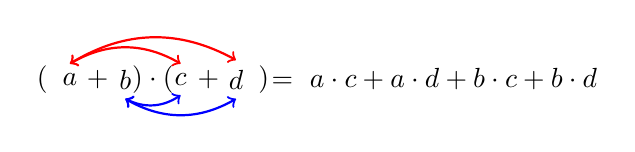
\begin{tikzpicture}[y=1em, x=1em,font=\sffamily]
    %% Draw the (a+b) part
    \node     at (0,0) {$($};
    \node (a) at (1,0) {$a$};
    \node     at (2,0) {$+$};
    \node (b) at (3,0) {$b$};
    \node     at (4,0) {$)\cdot($};

    %% Draw the *(c+d) part
    \node (c) at (5,0) {$c$};
    \node     at (6,0) {$+$};
    \node (d) at (7,0) {$d$};
    \node     at (8,0) {$)$};

    %% Draw the right hand side of the equation
    \node     at (14,0) {$~=~a\cdot c + a\cdot d + b\cdot c + b\cdot d$};

    %% Now make the pretty lines between the parts to FOIL
    \path[red,<->,thick] (a.north) edge[bend left] node {} (c.north);
    \path[red,<->,thick] (a.north) edge[bend left] node {} (d.north);

    \path[blue,<->,thick] (b.south) edge[bend right] node {} (c.south);
    \path[blue,<->,thick] (b.south) edge[bend right] node {} (d.south);

  \end{tikzpicture}

  \begin{subproblem}
  \item ${\displaystyle (x-3)^2}$
    \begin{eqnarray*}
      (x-3)^2 & = & (x-3)\cdot(x-3), \\
              & = & x\cdot x - 3\cdot x - 3\cdot x + (-3)\cdot(-3), \\
              & = & x^2 - 3x - 3x + 9, \\
              & = & x^2 - 6x + 9.
    \end{eqnarray*}
  \item ${\displaystyle (x+5)^2}$
    \vfill
  \item ${\displaystyle (y-4)^2}$
    \vfill
  \item ${\displaystyle (y+a)^2}$ where $a$ is a constant.
    \vfill
  \end{subproblem}
  
\item if $(x-a)^2=x^2+12x+36$ what is the value of $a$? (Briefly
  explain how you arrived at your result.)

  \vfill

\end{problem}


\actTitle{Quadratic Functions}
\begin{problem}

\item A traffic engineer observes the movement of traffic on a busy
  street. She estimates that when the density of cars is low the rate
  of flow is also low, and as the density increases the rate of flow
  increases. However, once the density of cars reaches a certain point
  the traffic slows, and the rate of flow begins to decrease.

  Some tests are run, and it is estimated that when the traffic
  density is 0 cars/meter that the rate of flow is 0 cars/minute. When
  the density is high, roughly 0.1 cars/meter or more, there is
  gridlock, and the rate of flow is 0 cars/minute. Finally, when there
  is 0.05 cars per meter the rate of flow is at a maximum of 20 cars
  per minute.
  
  \begin{subproblem}
  \item Assuming that the rate of flow is 0 if the density is greater
    than 0.1 make a rough sketch of the rate of flow as a function of
    the density of cars.
    \sideNote{Label your axes and properly annotate your graph.}
    \vfill
  \item Assuming that the rate of flow is a quadratic function of the
    traffic density when the density is between 0 and 0.1 cars/meter
    inclusive, determine the formula for the traffic density.
    \vfill
  \end{subproblem}

  \clearpage

\item Maximize the product of two positive numbers whose sum is five.
\begin{subproblem}
  \item The product of two numbers can be thought of as the area of a
    rectangle. Make a rough sketch of a rectangle.
    \sideNote{The product of two numbers is the area of a rectangle!}
    \vfill
  \item Within the sketch above, identify and label the variables
    that you will use.
  \item Determine the formula for the function to be maximized.
    \sideNote{This is called the "Cost Function." It should have two
      variables.}  
    \vfill
  \item Determine any other relevant relationships between your
    variables that must be true in all circumstances.  \sideNote{This
      is called the "Constraint." It should have two variables.}
    \vfill
  \item How will you solve this problem?
    \vfill
  \item Determine the values of the two numbers.
    \sideNote{Check your work and make sure that you maximized the
      profit and did not minimize it.}
    \vfill
    \vfill
\end{subproblem}

  \clearpage

\item A developer has a square plot of land that is 100 meters by 100
  meters, and the land is next to a river. The land will be divided
  into two parts. One part will be formed by cutting out a rectangle
  in one corner of the large plot, and its width will be along the
  river. The height of the rectangle will be ten meters shorter than
  its width.  It is estimated that this new rectangular plot of land
  will sell for \$2.00 per square meter plus 100\$/meter times the
  width. The remaining land will be sold for \$4.00 per square meter.
  Determine the dimensions of the rectangular plot that will result in
  the highest profit.

    \begin{subproblem}
      \item Make a sketch of the land with a corner designated for one
        of the plots.
        \sideNote{Label important aspects of the sketch.}
        \vfill
      \item Within the sketch above, identify and label the variables
        that you will use.
      \item Determine the total selling price for the land in terms of
        both variables.  \sideNote{This is called the "Cost Function."
          It should have at least two variables in it.}
        
        \vfill

        \clearpage

      \item Determine any other relevant relationships between your
        variables that must be true in all circumstances.
        \sideNote{This is called the "Constraint." It should have two
          variables in it.}  
        \vfill
      \item How will you solve this problem?
        \vspace{2em}
      \item Determine the dimensions of the rectangular plot that will
        result in the highest profit.
        \sideNote{Check your work and make sure that you maximized the
          profit and did not minimize it.}
        \vfill
        \vfill
    \end{subproblem}

\end{problem}

\postClass

\begin{problem}
\item Briefly state two ideas from today's class.
  \begin{itemize}
  \item
  \item
  \end{itemize}

\item Determine the vertex of the following parabolas.
  \begin{subproblem}
  \item $y=-x^2+10x-5$
  \item $y=2x^2-10x+18$
  \item $y=3x^2+4+1$
  \item $y=5x^2+2$
  \item $y=5x^2+x+2$
  \end{subproblem}

\item Two super hero capes will be sewn as part of a
  demonstration. One cape will be in the shape of a square. The other
  cape will be in the shape of a triangle, and the height is the same
  length as its base. They will be displayed together, and the sum of
  the two lengths must be 6 feet. What are the dimensions of the capes
  that will minimize the total area of the capes?
  \begin{subproblem}
  \item What are the steps you will take to solve this problem?
  \item Follow your steps and determine the dimensions of the two
    capes that will meet the given criteria.
  \end{subproblem}

\item Determine the numbers whose sum is 30 and their product is as
  large as possible. (Show your work and justify your answers
  mathematically.)

\item Two types of bacteria will be used to produce a medicinal
  compound. Bacteria A will be given $x$ hours, and it produces 3g of
  the compound per hour. Bacteria B will be given $y$ hours, and it
  produces 4g of the compound per hour. The total cost for the type A
  bacteria is $x^2$ dollars, and the total cost for the type B
  bacteria is $2y^2$ dollars. A total of 40g of product will be
  required. How many hours should be allocated to each bacteria to
  minimize the total cost

\item You have been asked to help design a channel taking water from a
  lake into a reservoir.  The channel must have a rectangular cross
  section with a fixed depth and width throughout its entire length.
  The bigger the cross section, the more the channel will cost.  In
  fact, the total cost of building the channel will be \$30,000
  dollars per meter of depth and \$10,000 per meter of width of its
  cross section, and the government has budgeted a total of \$100,000
  to construct the channel.  The government wants you to use this
  money to build a channel which will maximize the rate at which water
  flows through the channel (which is proportional to the cross
  sectional area of the channel).  What is the depth and width that
  will accomplish this?

\item Two chicken coops will be constructed using 120 feet of
  fencing. The coops will be in the shape of a rectangle with fencing
  across the middle dividing the rectangle into two equal
  rectangles. What dimensions will give the largest total area for the
  two coops?

\end{problem}


%%% Local Variables:
%%% mode: latex
%%% TeX-master: "../labManual"
%%% End:
